% =========================================================================
% Presentation of the article (English, Beamer, 16:9, highly visual):
% Full-Chain Multi-Hop Retrieval with Reified Assertion Graphs,
% Canonical Entity Memories, and Bounded Evidence Planning.
% Compile: tectonic presentacion_articulo_en.tex
% =========================================================================
\documentclass[aspectratio=169,10pt]{beamer}
\usepackage[T1]{fontenc}
\usepackage[utf8]{inputenc}
\usepackage{lmodern}
\usepackage{amsmath,amssymb}
\usepackage{booktabs}
\usepackage{tikz}
\usetikzlibrary{arrows.meta,positioning,fit,backgrounds,calc,shapes.geometric}
\usepackage{pgfplots}
\pgfplotsset{compat=1.17}

\usetheme{default}
\usecolortheme{seagull}
\definecolor{azul}{RGB}{31,80,154}
\definecolor{teja}{RGB}{186,84,32}
\definecolor{verde}{RGB}{34,120,74}
\definecolor{grisf}{RGB}{100,100,100}
\setbeamercolor{frametitle}{fg=azul}
\setbeamercolor{title}{fg=azul}
\setbeamercolor{structure}{fg=azul}
\setbeamertemplate{navigation symbols}{}
\setbeamertemplate{footline}[frame number]
\setbeamertemplate{itemize items}[circle]
\newcommand{\sys}{\textsc{CatRAG-Reif}}
\newcommand{\hippo}{HippoRAG~2}
\newcommand{\good}[1]{\textcolor{verde}{\textbf{#1}}}
\newcommand{\bad}[1]{\textcolor{teja}{\textbf{#1}}}
\DeclareMathOperator*{\Top}{Top}

\tikzset{
  caja/.style={draw=azul, rounded corners=2pt, align=center, inner sep=4pt, fill=azul!8, font=\scriptsize},
  dato/.style={draw=grisf, dashed, rounded corners=2pt, align=center, inner sep=3pt, font=\scriptsize},
  ent/.style={draw=azul, ellipse, align=center, inner sep=2pt, font=\scriptsize},
  aser/.style={draw=azul, rectangle, rounded corners=1pt, align=center, inner sep=3pt, fill=azul!12, font=\scriptsize},
  chk/.style={draw=grisf, rectangle, align=center, inner sep=3pt, font=\scriptsize},
  fl/.style={-{Stealth[length=2mm]}, semithick, azul},
  flbad/.style={-{Stealth[length=2mm]}, semithick, teja},
  flok/.style={-{Stealth[length=2mm]}, semithick, verde},
  et/.style={font=\tiny, text=grisf, align=center},
}

\title{Full-Chain Multi-Hop Retrieval with Reified Assertion Graphs,\\
Canonical Entity Memories, and Bounded Evidence Planning}
\subtitle{Evaluation under strict model parity on 2WikiMultihopQA and HotpotQA}
\author{}
\date{September 2026}

\begin{document}

\begin{frame}
\titlepage
\vspace{-6mm}
\centering\scriptsize
$\mathrm{FC@}5$: \textbf{97.7} vs.\ 65.8 (\hippo{}) / 67.6 (CatRAG) on 2Wiki
\;·\; \textbf{93.0} vs.\ 80.4 on HotpotQA, zero tuning \;·\; ${\sim}\$0.001$/query
\end{frame}

\begin{frame}{Roadmap}
\begin{enumerate}
\item \textbf{The problem}: chains break while recall looks fine --- and its two structural causes.
\item \textbf{The representation}: reified assertions over canonical entities; an audited memory; a layered graph with a closed-form walk.
\item \textbf{The planner}: three LLM roles under contracts --- analyst, repair hop, set packer.
\item \textbf{The evidence}: parity protocol, main results, depth analysis, ablations, a no-graph control, and the system's evolution.
\end{enumerate}
\vfill
\scriptsize Every number in this talk is a single pre-registered measurement,
paired per question with bootstrap CIs; every LLM call is cached (zero-cost
reproduction).
\end{frame}

% =========================== PART 1: PROBLEM ============================
\begin{frame}{The problem: high recall, broken chains}
\begin{columns}[T]
\column{0.52\textwidth}
The task metric must be the \textbf{complete chain}:
\[
\mathrm{R@}k=\frac{|G_q\cap T_k(q)|}{|G_q|},\qquad
\mathrm{FC@}k=\mathbf 1\bigl[G_q\subseteq T_k(q)\bigr]
\]
A reader cannot compose an answer from $3$ of $4$ passages:
$\mathrm{R@}5=0.75$ is \emph{operationally zero}.
\vspace{1mm}
\begin{center}\small
\begin{tabular}{lcc}
\toprule
double-bridge stratum (2Wiki) & R@5 & FC@5\\
\midrule
BM25 & $50.9$ & \bad{$0.9$}\\
\hippo{} (its code, our run) & --- & \bad{$12.3$}\\
\bottomrule
\end{tabular}
\end{center}
\column{0.46\textwidth}
\centering
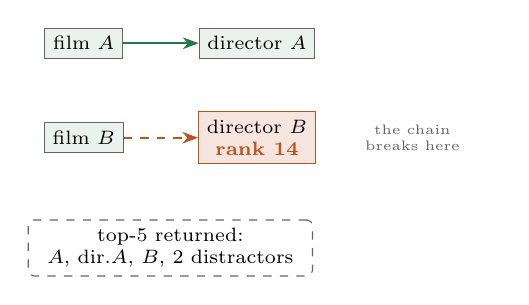
\begin{tikzpicture}[x=1mm,y=1mm,font=\tiny]
  \node[chk, fill=verde!10] (g1) at (0,30) {film $A$};
  \node[chk, fill=verde!10] (g2) at (22,30) {director $A$};
  \node[chk, fill=verde!10] (g3) at (0,18) {film $B$};
  \node[chk, fill=teja!15, draw=teja] (g4) at (22,18) {director $B$\\ \bad{rank 14}};
  \node[dato, text width=34mm] (top) at (11,4) {top-5 returned:\\ $A$, dir.$A$, $B$, 2 distractors};
  \draw[flok] (g1)--(g2); \draw[flbad, dashed] (g3)--(g4);
  \node[et, right=1mm of g4, text width=20mm]{the chain\\ breaks here};
\end{tikzpicture}

\vspace{2mm}
\scriptsize The signature of the state of the art: \emph{partial} recall
stays high while the set misses exactly the bridge passage.
\end{columns}
\end{frame}

\begin{frame}{Two structural causes, both measured}
\begin{columns}[T]
\column{0.5\textwidth}
\textbf{1 · Identity unresolved at indexing.}
\begin{center}
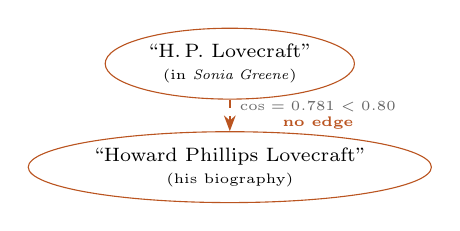
\begin{tikzpicture}[node distance=4mm]
  \node[ent, draw=teja] (m1) {``H.\,P. Lovecraft''\\ \tiny(in \emph{Sonia Greene})};
  \node[ent, draw=teja, below=of m1] (m2) {``Howard Phillips Lovecraft''\\ \tiny(his biography)};
  \draw[flbad, dashed] (m1) -- node[et, right]{$\cos=0.781<0.80$\\ \bad{no edge}} (m2);
\end{tikzpicture}
\end{center}
\scriptsize Thresholded synonymy ($172$k edges in \hippo{}) fails where it
is most needed: \bad{57\% of chain failures were identity islands}.
\column{0.5\textwidth}
\textbf{2 · Resources fixed per query.}
\begin{itemize}\footnotesize
\item one $\le 4$-triple selection budget,
\item one seed distribution,
\item one slack position in the top-5,
\end{itemize}
\emph{shared} across all chains of the question. A double chain is starved
\textbf{by construction}: covering one branch guarantees $\mathrm{FC}=0$
regardless of ranking quality.
\vspace{2mm}

\scriptsize Both causes are properties of the \emph{design}, not of model
quality --- so both are removable by design.
\end{columns}
\end{frame}

\begin{frame}{Contributions}
\begin{enumerate}
\item \textbf{Reified-assertion graph over canonical entities} --- facts as
  first-class, query-modulable nodes; identity resolved \emph{before} the
  graph; no synonymy edges.
\item \textbf{Audited entity memory} --- merge decisions with provenance,
  audited against external Wikidata gold: over-merges $74\to32$.
\item \textbf{Bounded evidence planner} --- analyst / repair / packer under
  JSON contracts; $\le 3$ LLM calls; deterministic control flow.
\item \textbf{Structural analysis} --- the layered walk has a closed form:
  \emph{the walk cannot chain hops; the seeding does}.
\item \textbf{Evidence} --- strict parity, paired statistics, ablations,
  a no-graph control, a depth (accumulation-vs-collapse) analysis, and
  frozen-configuration generalization.
\end{enumerate}
\end{frame}

\begin{frame}{Architecture and notation: pay once at indexing, decide well at query time}
\begin{columns}[T]
\column{0.55\textwidth}
\footnotesize
\textbf{Indexing} (once per corpus, no questions):
passages $\mathcal C$ $\to$ assertions $\mathcal A$ (extraction) $\to$
entities $\mathcal E$ (canonical memory) $\to$ graph
$G=(\mathcal C\cup\mathcal E\cup\mathcal A, E)$ $+$ aligned vector stores
$e(\tau_a)$, $\phi(\varepsilon)$, $e(c)$.

\textbf{Query} (8 steps, $\le3$ LLM calls): affinity $\sigma$; linking
$L(q)$; analyst (plan, $S(q)$, slots); seeding $\mathbf v$; modulation
$\mu$; walk $\mathbf p^{*}$; conditional repair; set packing.

\vspace{1mm}
Real sizes (2Wiki): $6{,}119$ passages $\to$ $47{,}999$ assertions,
$27{,}966$ entities, $165$k edges; ${\sim}\$3$, once.
\column{0.43\textwidth}
\centering
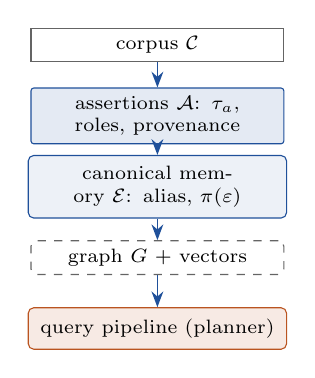
\begin{tikzpicture}[x=1mm,y=1mm,font=\tiny]
  \node[chk, text width=30mm] (c) at (18,38) {corpus $\mathcal C$};
  \node[aser, text width=30mm] (a) at (18,29) {assertions $\mathcal A$: $\tau_a$, roles, provenance};
  \node[caja, text width=30mm] (e) at (18,20) {canonical memory $\mathcal E$: alias, $\pi(\varepsilon)$};
  \node[dato, text width=30mm] (g) at (18,11) {graph $G$ $+$ vectors};
  \node[caja, fill=teja!12, draw=teja, text width=30mm] (q) at (18,2) {query pipeline (planner)};
  \draw[fl] (c)--(a); \draw[fl] (a)--(e); \draw[fl] (e)--(g); \draw[fl] (g)--(q);
\end{tikzpicture}
\end{columns}
\end{frame}

% ====================== PART 2: REPRESENTATION ==========================
\begin{frame}{Representation I: the fact as a node, not an edge}
\centering
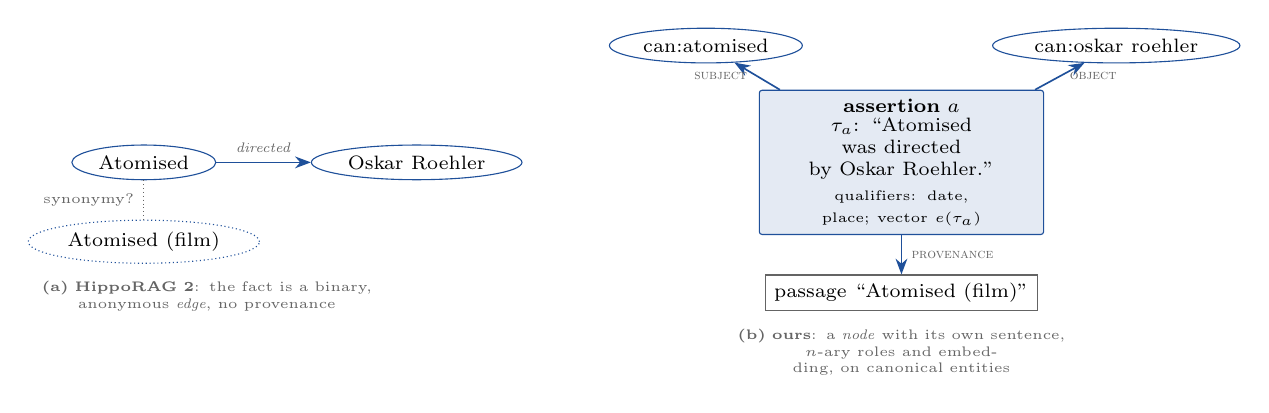
\begin{tikzpicture}[node distance=4mm and 8mm]
  \node[ent] (t1) {Atomised};
  \node[ent, right=12mm of t1] (t2) {Oskar Roehler};
  \draw[fl] (t1) -- node[et, above]{\emph{directed}} (t2);
  \node[ent, below=5mm of t1, densely dotted] (t3) {Atomised (film)};
  \draw[grisf, densely dotted] (t1) -- node[et, left]{synonymy?} (t3);
  \node[et, below=1mm of t3, xshift=8mm, text width=42mm]
    {\textbf{(a) \hippo{}}: the fact is a binary,\\ anonymous \emph{edge}, no provenance};
  \node[aser, right=30mm of t2, text width=34mm] (a) {\textbf{assertion} $a$\\[-1pt]
    $\tau_a$: ``Atomised was directed\\ by Oskar Roehler.''\\[1pt]
    {\tiny qualifiers: date, place; vector $e(\tau_a)$}};
  \node[ent, above left=4mm and -2mm of a] (e1) {can:atomised};
  \node[ent, above right=4mm and -2mm of a] (e2) {can:oskar roehler};
  \node[chk, below=5mm of a] (c1) {passage ``Atomised (film)''};
  \draw[fl] (a) -- node[et, left]{\textsc{subject}} (e1);
  \draw[fl] (a) -- node[et, right]{\textsc{object}} (e2);
  \draw[fl] (a) -- node[et, right]{\textsc{provenance}} (c1);
  \node[et, below=1mm of c1, text width=48mm]
    {\textbf{(b) ours}: a \emph{node} with its own sentence,\\ $n$-ary roles and embedding, on canonical entities};
\end{tikzpicture}
\vspace{1mm}
\begin{itemize}\footnotesize
\item We embed \textbf{the sentence}, not the label: robust to extractor
  noise; the datum the question compares (dates, doses) travels \emph{inside}
  the retrievable unit.
\item The walk reasons \textbf{through the fact} and its transit is
  per-query: $\mu_a=\tfrac14+\tfrac34\,\tilde\sigma_a(q)$.
\end{itemize}
\end{frame}

\begin{frame}{Representation II: why the assertion-node matters (three properties)}
\begin{columns}[T]
\column{0.55\textwidth}
\begin{enumerate}\footnotesize
\item \textbf{Query modulability.} A triple graph fixes the transition
  distribution at indexing; CatRAG re-weights the same binary support. Here
  each fact is \emph{addressable}: $P(\varepsilon\!\to\!a)\propto\mu_a(q)$,
  approved facts transit at full weight.
\item \textbf{$n$-ary closure.} Triples force binarity; extra participants
  and qualifiers are lost. The assertion keeps them in $\tau_a$ and its
  roles.
\item \textbf{Sentence semantics.} Affinity on $e(\tau_a)$, a
  self-contained sentence --- not a concatenation of noisy labels.
\end{enumerate}
\column{0.43\textwidth}
\centering
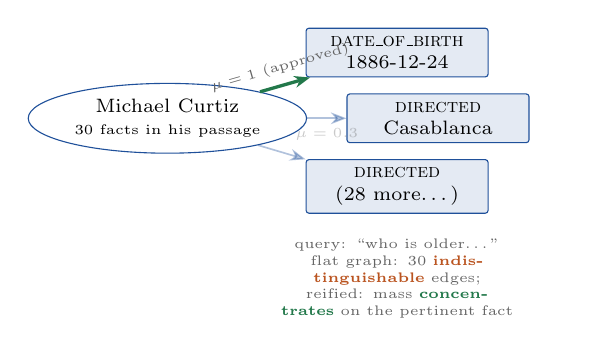
\begin{tikzpicture}[node distance=1.2mm and 2mm, font=\tiny]
  \node[ent] (c) {Michael Curtiz\\ \tiny 30 facts in his passage};
  \node[aser, above right=2mm and 5mm of c, text width=21mm] (h1) {\textsc{date\_of\_birth}\\ 1886-12-24};
  \node[aser, right=5mm of c, text width=21mm] (h2) {\textsc{directed}\\ Casablanca};
  \node[aser, below right=2mm and 5mm of c, text width=21mm] (h3) {\textsc{directed}\\ (28 more\dots)};
  \draw[flok, very thick] (c) -- node[et, above, sloped]{$\mu=1$ (approved)} (h1);
  \draw[fl, opacity=0.35] (c) -- node[et, below, sloped]{$\mu=0.3$} (h2);
  \draw[fl, opacity=0.35] (c) -- (h3);
  \node[et, below=2mm of h3, text width=40mm]
    {query: ``who is older\dots''\\
     flat graph: 30 \bad{indistinguishable} edges;\\
     reified: mass \good{concentrates} on the pertinent fact};
\end{tikzpicture}
\end{columns}
\end{frame}

\begin{frame}{Canonical entity memory: kill the islands in the index}
\begin{columns}[T]
\column{0.48\textwidth}
\centering
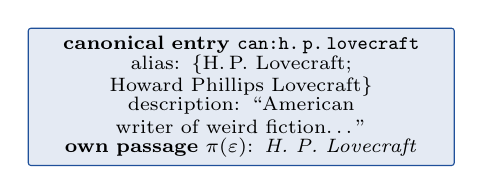
\begin{tikzpicture}[node distance=3mm]
  \node[aser, text width=52mm] (f) {\textbf{canonical entry} \texttt{can:h.\,p.\,lovecraft}\\[-1pt]
   alias: \{H.\,P. Lovecraft; Howard Phillips Lovecraft\}\\[-1pt]
   description: ``American writer of weird fiction\dots''\\[-1pt]
   \textbf{own passage} $\pi(\varepsilon)$: \emph{H. P. Lovecraft}};
\end{tikzpicture}
\vspace{1mm}

\footnotesize Mention cards (name $+$ context) $\to$ candidates on 2
channels $\to$ hard constraints (dates, ordinals, disambiguators) $\to$
LLM adjudication (strict: relatives, successors, remakes are \emph{not} the
same) $\to$ transitive closure. Built \textbf{once, from the corpus only}.
\column{0.5\textwidth}
Per-pair decision (name channel $\nu$, context channel $\phi$, hard
constraints $H$):
\[
d(m,m')=\begin{cases}
\textsc{veto} & \neg H\\
\textsc{merge} & \operatorname{fold}(\nu_m){=}\operatorname{fold}(\nu_{m'})\\
\textsc{merge} & \langle\nu,\nu'\rangle{\ge}0.90 \wedge \langle\phi,\phi'\rangle{\ge}0.70\\
\textsc{judge} & \langle\nu,\nu'\rangle{\ge}0.80 \vee (\langle\phi,\phi'\rangle{\ge}0.75 \wedge \text{tok})\\
\textsc{drop} & \text{otherwise}
\end{cases}
\]
\footnotesize $40{,}276$ mentions $\to$ $27{,}966$ entries; $178/188$
diagnosed islands resolved; the canonical graph needs \textbf{no synonymy
edges at all}.
\end{columns}
\end{frame}

\begin{frame}{The memory is audited against external gold (Wikidata QIDs)}
\begin{columns}[T]
\column{0.52\textwidth}
\footnotesize
2Wiki carries QIDs for its evidence entities (never used to build). Unit:
(surface form, QID) of chain entities.
\begin{itemize}\footnotesize
\item entry with $2$ QIDs of distinct forms $=$ \textbf{over-merge};
\item QID split across entries $=$ \textbf{under-merge};
\item every union carries \textbf{provenance} $\Rightarrow$ each over-merge
  is attributed to the rule that bridged it.
\end{itemize}
\begin{center}\small
\begin{tabular}{lccc}
\toprule
memory & over & under & dominant bridge\\
\midrule
initial & $74/2{,}211$ & $6$ & title$\to$subject union\\
curated & \good{$\mathbf{32}$} & $6$ & residual judge errors\\
\bottomrule
\end{tabular}
\end{center}
\column{0.46\textwidth}
\footnotesize
\textbf{Four registered decisions} (no silent patches):
\begin{enumerate}\footnotesize
\item title$\to$subject unions with a genuine title mention $\to$ judge
  (rejected $893/1{,}549$);
\item near-identical names with differing parenthetical disambiguators
  $\to$ judge (``X (1922 film)'' $\ne$ ``X (1923 film)'');
\item title cards inherit the article subject's dates;
\item provenance stored per union.
\end{enumerate}
\emph{Honesty note}: two dev questions relied on \bad{fortunate wrong
merges} (a dataset-mislabeled homonym; an emperor merged with his son).
We give them up: identity precision is the foundation.
\end{columns}
\end{frame}

\begin{frame}{The search graph is layered --- and its walk has a closed form}
\begin{columns}[T]
\column{0.5\textwidth}
\footnotesize
\textbf{Proposition.} Entities have in-degree $0$; each assertion drains
into its unique source passage; passages are sinks. Hence
\[
\mathbf p^{*}(c)=\beta\Bigl[\mathbf v(c)
+\lambda\!\!\sum_{\varepsilon: c\in N(\varepsilon)}\!\!\tfrac{\mathbf v(\varepsilon)}{Z_\varepsilon}
+\lambda^{2}\!\!\sum_{\varepsilon}\sum_{\substack{a\ni\varepsilon\\ c(a)=c}}\tfrac{\mathbf v(\varepsilon)\mu_a}{Z_\varepsilon}\Bigr]
\]
verified numerically to the 4th decimal.
\vspace{1mm}

\textbf{Consequence}: the walk \emph{diffuses} the seeds one fact away;
it \bad{cannot chain hops}. Multi-hop capability must live in
\good{which entities and own passages get seeded} --- the planner's job.
\column{0.48\textwidth}
\centering
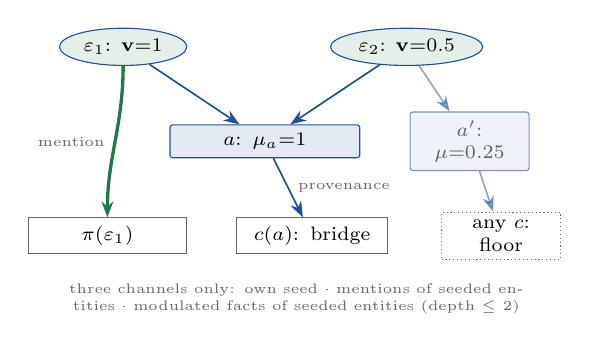
\begin{tikzpicture}[x=1mm,y=1mm,font=\tiny]
  \node[ent, fill=verde!12] (e1) at (8,28) {$\varepsilon_1$: $\mathbf v{=}1$};
  \node[ent, fill=verde!12] (e2) at (44,28) {$\varepsilon_2$: $\mathbf v{=}0.5$};
  \node[aser, text width=22mm] (a1) at (26,16) {$a$: $\mu_a{=}1$};
  \node[aser, text width=13mm, opacity=0.6] (a2) at (52,16) {$a'$: $\mu{=}0.25$};
  \node[chk, text width=18mm] (c1) at (6,4) {$\pi(\varepsilon_1)$};
  \node[chk, text width=17mm] (c2) at (32,4) {$c(a)$: bridge};
  \node[chk, densely dotted, text width=13mm] (c3) at (56,4) {any $c$: floor};
  \draw[fl] (e1)--(a1); \draw[fl] (e2)--(a1); \draw[fl, opacity=0.5] (e2)--(a2);
  \draw[fl] (a1)-- node[et,right]{provenance} (c2);
  \draw[fl, opacity=0.5] (a2)--(c3);
  \draw[flok, very thick] (e1) to[out=-90,in=90] node[et,left]{mention} (c1);
  \node[et, text width=58mm] at (30,-4)
   {three channels only: own seed · mentions of seeded entities · modulated
    facts of seeded entities (depth $\le 2$)};
\end{tikzpicture}
\vspace{1mm}

\scriptsize Iterative solver kept only for cyclic variants (synonymy;
clinical \textsc{is-a} layers).
\end{columns}
\end{frame}

% ========================= PART 3: PLANNER ==============================
\begin{frame}{The query pipeline: Algorithm 1 on the graph}
\begin{columns}[T]
\column{0.5\textwidth}
\footnotesize
\begin{enumerate}\footnotesize
\item $\sigma_a=\langle e(q),e(\tau_a)\rangle$ (one matrix product).
\item Link mentions $\to L(q)\subseteq\mathcal E$.
\item \textbf{Analyst} on $\Top_{40}\sigma\cup\text{frontier}(L)$: plan,
  selection $S(q)$ ($\tilde\sigma_S{=}1$), unfilled slots. \hfill{\tiny LLM 1}
\item Seed $\mathbf v$ (Eq.\ next slide).
\item Modulate $\tilde A=A\,\mathrm{diag}(\mu)$; $P=D^{-1}\tilde A$.
\item Walk to $\mathbf p^{*}$
  ($\lambda{=}0.5$, $\lVert\Delta\rVert_1{<}10^{-9}$).
\item Slots left $\to$ \textbf{repair hop}, re-seed, re-walk
  ($\le3$ rounds). \hfill{\tiny LLM 2}
\item \textbf{Pack} the 5-set that covers the plan. \hfill{\tiny LLM 3}
\end{enumerate}
\column{0.48\textwidth}
\centering
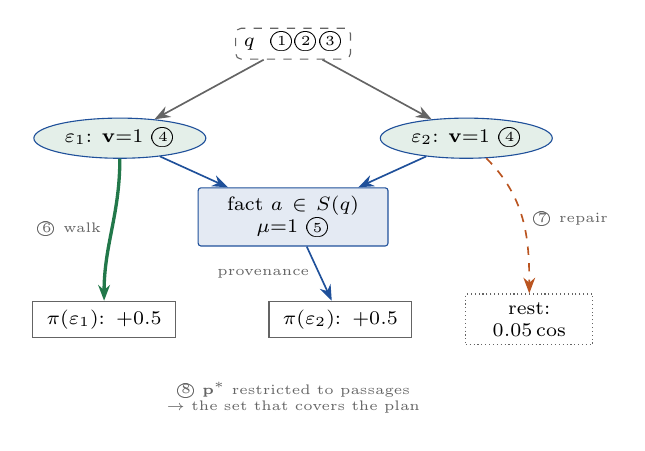
\begin{tikzpicture}[x=1mm, y=1mm, font=\tiny]
  \node[dato] (q)  at (32,42) {$q$ \ \textcircled{\tiny 1}\textcircled{\tiny 2}\textcircled{\tiny 3}};
  \node[ent, fill=verde!12] (e1) at (10,30) {$\varepsilon_1$: $\mathbf v{=}1$ \textcircled{\tiny 4}};
  \node[ent, fill=verde!12] (e2) at (54,30) {$\varepsilon_2$: $\mathbf v{=}1$ \textcircled{\tiny 4}};
  \node[aser, text width=22mm] (aa) at (32,20) {fact $a\in S(q)$\\ $\mu{=}1$ \textcircled{\tiny 5}};
  \node[chk, text width=16mm] (c1) at (8,7) {$\pi(\varepsilon_1)$: $+0.5$};
  \node[chk, text width=16mm] (c2) at (38,7) {$\pi(\varepsilon_2)$: $+0.5$};
  \node[chk, densely dotted, text width=14mm] (cx) at (62,7) {rest: $0.05\cos$};
  \draw[fl, grisf] (q)--(e1); \draw[fl, grisf] (q)--(e2);
  \draw[fl] (e1)--(aa); \draw[fl] (e2)--(aa);
  \draw[fl] (aa)-- node[et,left]{provenance} (c2);
  \draw[flok, very thick] (e1) to[out=-90,in=90] node[et,left]{\textcircled{\tiny 6} walk} (c1);
  \draw[flbad, dashed] (e2) to[out=-45,in=90] node[et,right]{\textcircled{\tiny 7} repair} (cx);
  \node[et, text width=58mm] at (32,-3)
   {\textcircled{\tiny 8} $\mathbf p^{*}$ restricted to passages $\to$ the set that covers the plan};
\end{tikzpicture}
\end{columns}
\end{frame}

\begin{frame}{The analyst: plan the chain \emph{before} selecting}
\footnotesize
\emph{``Which film has the director died first, B\'il\'a Spona or A Night at Earl Carroll's?''}
\centering
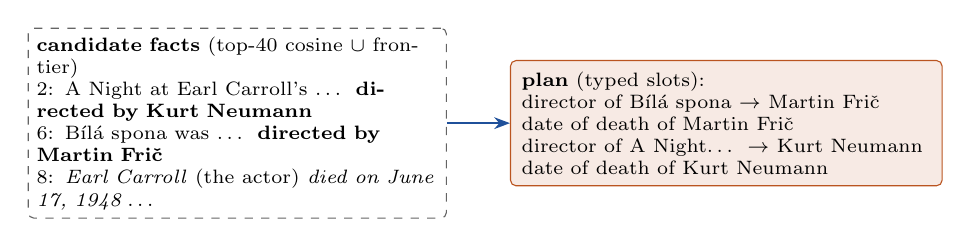
\begin{tikzpicture}[node distance=2.5mm and 8mm]
  \node[dato, text width=51mm, align=left] (cand) {\textbf{candidate facts} (top-40 cosine $\cup$ frontier)\\
    2: A Night at Earl Carroll's \dots{} \textbf{directed by Kurt Neumann}\\
    6: B\'il\'a spona was \dots{} \textbf{directed by Martin Fri\v{c}}\\
    8: \emph{Earl Carroll} (the actor) \emph{died on June 17, 1948}\,\dots};
  \node[caja, right=of cand, fill=teja!12, draw=teja, text width=52mm, align=left] (plan) {\textbf{plan} (typed slots):\\
    director of B\'il\'a spona $\to$ Martin Fri\v{c}\\
    date of death of Martin Fri\v{c}\\
    director of A Night\dots{} $\to$ Kurt Neumann\\
    date of death of Kurt Neumann};
  \draw[fl] (cand) -- (plan);
\end{tikzpicture}
\vspace{1.5mm}
\begin{columns}[T]
\column{0.55\textwidth}
\textbf{Without a plan} (direct selector, fixed budget 4):\\
\bad{picked the actor Earl Carroll as ``director''} and omitted Kurt
Neumann \emph{who was on the list} $\Rightarrow$ broken chain.
\column{0.45\textwidth}
\textbf{With a plan} (budget $=$ number of slots):\\
\good{selects both bridge facts}; hard rule: slots may name an entity
\emph{only if a candidate fact states it} --- else $[X]$; parametric
knowledge forbidden.
\end{columns}
\vspace{1.5mm}
The same call performs \textbf{entity recognition} (mentions $\to$
canonical form $\to$ memory) and declares the \textbf{unfilled slots} that
feed the repair hop.
\end{frame}

\begin{frame}{The analyst for real: raw input/output on a benchmark question}
\scriptsize
\textbf{Input} (question $+$ 43 numbered facts $=\Top_{40}\sigma\,\cup$ 3 from the frontier):\\[0.5mm]
\texttt{Question: Do Walfredo Reyes Jr. and Zac Dysert have the same nationality}\\
\texttt{0: Walfredo Reyes Jr. was born on December 18, 1955.}\;
\texttt{\dots}\;
\texttt{17: Zac Dysert is an American football quarterback.}\;\texttt{\dots}\\[1mm]
\textbf{Raw output} (JSON mode, temperature 0, cached):
\begin{center}
\scriptsize
\fbox{\parbox{0.9\textwidth}{\texttt{\{"mentions": [\{"text": "Walfredo Reyes Jr.", "canonical": "Walfredo Reyes Jr."\}, \dots],\\
"plan": ["nationality of Walfredo Reyes Jr.", "nationality of Zac Dysert"],\\
"selected": [17, 18],\quad
"unfilled": [\{"query": "nationality of Walfredo Reyes Jr.", "anchor": "Walfredo Reyes Jr."\}]\}}}}
\end{center}
\vspace{1mm}
\textbf{Deterministic post-processing} (the LLM only writes text and copies
line numbers):
\begin{itemize}\scriptsize
\item \texttt{selected} are \emph{local} indices $\to$ guarded map to global
  assertion ids ($17\to$ \texttt{Zac Dysert::a1}); dedup; dynamic cap
  $\min(8,\max(2,|\text{plan}|))$;
\item \texttt{canonical} forms $\to$ linker $\to$ canonical entries (extends
  $L(q)$); \texttt{anchor} $\to$ entry $\to$ own passage $\to$ its
  assertions (repair candidates);
\item invalid indices / malformed JSON degrade gracefully (guards; dense
  fallback) --- thousands of calls per benchmark, zero hard failures.
\end{itemize}
\end{frame}

\begin{frame}{Seeding: four sources, one equation, observed values}
\vspace{-1mm}
\[
\mathbf v(u)=
\underbrace{\mathbb 1[u\in\mathcal E_S]\,\overline{\tilde\sigma}(u)}_{\text{hard gate}}
+\underbrace{\mathbb 1[u\in\mathcal C]\, w_{\text{pas}}\hat s(u)}_{\text{dense floor}}
+\underbrace{\epsilon\,\mathbb 1[u\in\Top_2\langle e(q),\phi\rangle]}_{\text{weak anchors}}
+\underbrace{\mathbb 1[u{=}\pi(\varepsilon)]\, w_{\text{link}}\mathbf v(\varepsilon)}_{\text{own passage}}
\]
\begin{columns}[T]
\column{0.56\textwidth}
\centering
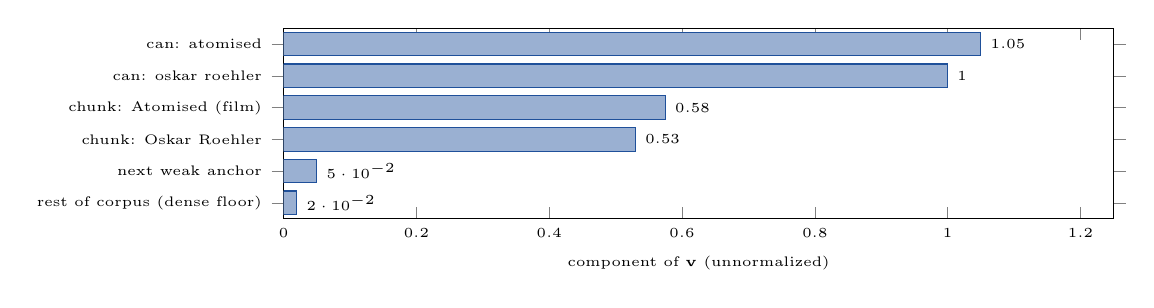
\begin{tikzpicture}
\begin{axis}[xbar, width=\textwidth, height=40mm, xmin=0, xmax=1.25,
  symbolic y coords={{rest of corpus (dense floor)},{next weak anchor},{chunk: Oskar Roehler},{chunk: Atomised (film)},{can: oskar roehler},{can: atomised}},
  ytick=data, xlabel={\tiny component of $\mathbf v$ (unnormalized)},
  nodes near coords, every node near coord/.append style={font=\tiny},
  tick label style={font=\tiny}, label style={font=\tiny}, bar width=3mm]
\addplot[fill=azul!45, draw=azul] coordinates {(0.02,{rest of corpus (dense floor)}) (0.05,{next weak anchor}) (0.530,{chunk: Oskar Roehler}) (0.575,{chunk: Atomised (film)}) (1.00,{can: oskar roehler}) (1.05,{can: atomised})};
\end{axis}
\end{tikzpicture}
\column{0.42\textwidth}
\footnotesize
Trace: \emph{``Who is the mother of the director of film Atomised?''}
\begin{itemize}\footnotesize
\item \texttt{can:oskar roehler} $=1.0$: entity of the approved fact ---
  \good{discovered}, not named in the question;
\item both \emph{own passages} get $0.5\cdot\mathbf v(\varepsilon)$;
\item dense floor: $94$--$98\%$ of raw mass, but ${\sim}1.6{\cdot}10^{-4}$
  per passage after normalization; a gated entity concentrates
  $25$--$60\times$ that.
\end{itemize}
After the walk: $p^{*}$(Atomised)$=0.0084$, $p^{*}$(Roehler)$=0.0063$,
first distractor $0.0004$ --- an order of magnitude.
\end{columns}
\end{frame}

\begin{frame}{Modulated personalized PageRank}
\[
\tilde A = A\,\operatorname{diag}(\mu),\qquad
\mu_u=\begin{cases}\tfrac14+\tfrac34\operatorname{clip}_{[0,1]}(\tilde\sigma_u)& u\in\mathcal A\\ 1&\text{else}\end{cases}
\qquad P=D^{-1}\tilde A
\]
\[
\mathbf p^{(t+1)}=\lambda\bigl(P^{\!\top}\mathbf p^{(t)}+m_{\text{dang}}\mathbf v\bigr)+(1-\lambda)\mathbf v,
\qquad \lambda=0.5
\]
\begin{itemize}\footnotesize
\item Columns entering \emph{assertion} nodes are rescaled: crossing a fact
  costs according to \emph{this} question; approved facts transit at
  $\mu=1$, irrelevant ones at the $0.25$ floor (never blocked).
\item Sinks (passages) recycle their mass to the seeds ($m_{\text{dang}}$):
  a page ``votes'' and restarts.
\item Dials ($\lambda{=}0.5$, $w_{\text{pas}}{=}0.05$, all-passage seeding)
  are \hippo{}'s published values --- \textbf{pre-registered parity}, frozen
  across datasets.
\item Sparse products over $165$k edges: milliseconds; no LLM.
\end{itemize}
\end{frame}

\begin{frame}{The repair hop: structural candidates beat cosine where cosine is blind}
\centering
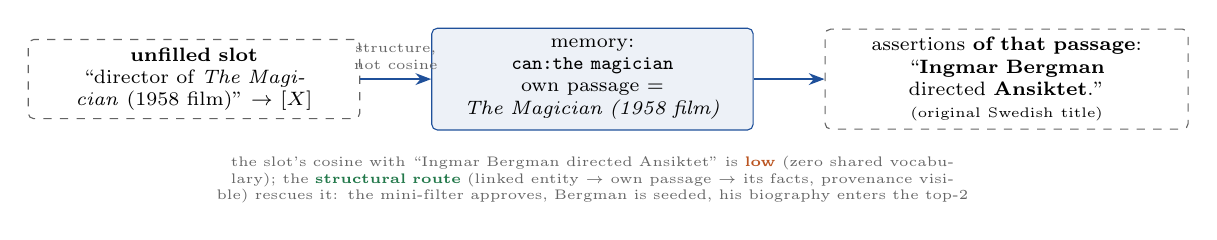
\begin{tikzpicture}[node distance=3mm and 9mm]
  \node[dato, text width=40mm] (hueco) {\textbf{unfilled slot}\\ ``director of \emph{The Magician} (1958 film)'' $\to$ $[X]$};
  \node[caja, right=of hueco, text width=38mm] (dicc) {memory:\\ \texttt{can:the magician}\\ own passage $=$\\ \emph{The Magician (1958 film)}};
  \node[dato, right=of dicc, text width=44mm] (hechos) {assertions \textbf{of that passage}:\\
    ``\textbf{Ingmar Bergman} directed \textbf{Ansiktet}.''\\ \tiny(original Swedish title)};
  \draw[fl] (hueco) -- node[et, above]{structure,\\ not cosine} (dicc);
  \draw[fl] (dicc) -- (hechos);
  \node[et, below=2mm of dicc, text width=104mm]
   {the slot's cosine with ``Ingmar Bergman directed Ansiktet'' is \bad{low}
    (zero shared vocabulary); the \good{structural route} (linked entity
    $\to$ own passage $\to$ its facts, provenance visible) rescues it: the
    mini-filter approves, Bergman is seeded, his biography enters the top-2};
\end{tikzpicture}
\vspace{2mm}
\begin{itemize}\footnotesize
\item Runs only if the plan left slots ($\sim$15--25\% of queries); up to 3
  rounds with re-planning when $[X]$ placeholders remain.
\item The genuinely new capability: bridges \textbf{immune to aliasing}
  (languages, original titles) --- unreachable for similarity and synonymy.
\end{itemize}
\end{frame}

\begin{frame}{Set packing, and the census of LLM roles}
\begin{columns}[T]
\column{0.44\textwidth}
\footnotesize
\textbf{Set packing} (LLM call 3): FC@$k$ is a property of the \emph{set}.
From the walk's top-12, pick the 5 that jointly cover the plan (walk's
top-2 preserved). Worth $+1.5$ FC@5 and $+6$ FC@2 on the probe; $+4.0$
R@2 on HotpotQA.
\vspace{2mm}

\textbf{Bounded agency}: JSON contracts validated; $\le3$ calls/query;
read-only tools; cache by (model, prompt); deterministic control flow ---
\emph{the LLM decides within contracts; the algorithm keeps control.}
\column{0.54\textwidth}
\centering
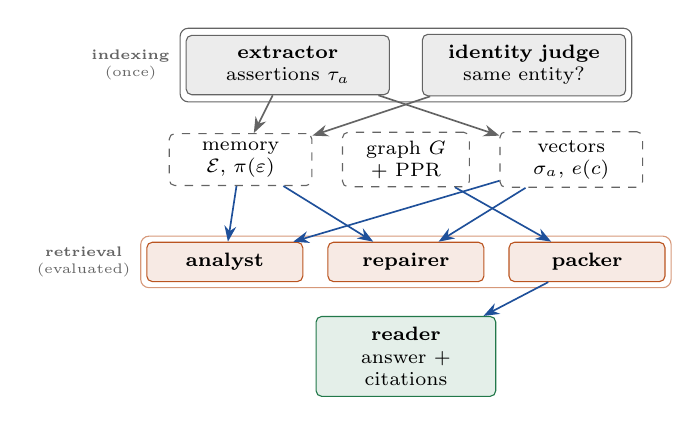
\begin{tikzpicture}[x=1mm, y=1mm, font=\tiny]
  \node[caja, fill=grisf!12, draw=grisf, text width=23mm] (x1) at (13,46) {\textbf{extractor}\\ assertions $\tau_a$};
  \node[caja, fill=grisf!12, draw=grisf, text width=23mm] (x2) at (43,46) {\textbf{identity judge}\\ same entity?};
  \node[dato, text width=16mm] (h1) at (7,34)  {memory\\ $\mathcal E$, $\pi(\varepsilon)$};
  \node[dato, text width=14mm] (h2) at (28,34) {graph $G$\\ $+$ PPR};
  \node[dato, text width=16mm] (h3) at (49,34) {vectors\\ $\sigma_a$, $e(c)$};
  \draw[fl, grisf] (x1)--(h1); \draw[fl, grisf] (x1)--(h3); \draw[fl, grisf] (x2)--(h1);
  \node[caja, fill=teja!12, draw=teja, text width=17mm] (r1) at (5,21)  {\textbf{analyst}};
  \node[caja, fill=teja!12, draw=teja, text width=17mm] (r2) at (28,21) {\textbf{repairer}};
  \node[caja, fill=teja!12, draw=teja, text width=17mm] (r3) at (51,21) {\textbf{packer}};
  \draw[fl] (h1)--(r1); \draw[fl] (h3)--(r1); \draw[fl] (h1)--(r2); \draw[fl] (h3)--(r2); \draw[fl] (h2)--(r3);
  \node[caja, fill=verde!12, draw=verde, text width=20mm] (l1) at (28,9) {\textbf{reader}\\ answer $+$ citations};
  \draw[fl] (r3)--(l1);
  \begin{scope}[on background layer]
    \node[fit=(x1)(x2), draw=grisf, rounded corners=3pt, inner sep=2pt,
      label={[et]left:{\textbf{indexing}\\ (once)}}] {};
    \node[fit=(r1)(r3), draw=teja!60, rounded corners=3pt, inner sep=2pt,
      label={[et]left:{\textbf{retrieval}\\ (evaluated)}}] {};
  \end{scope}
\end{tikzpicture}
\end{columns}
\end{frame}

% ========================= PART 4: EVIDENCE =============================
\begin{frame}{Protocol: strict parity, data separation, pre-registration}
\begin{columns}[T]
\column{0.52\textwidth}
\footnotesize
\textbf{Parity.} Same backbone everywhere
(\texttt{gpt-4o-mini}$+$\texttt{te3-small}); \hippo{} run \emph{with its
official code} on the same corpus; CatRAG compared on its published numbers
under the identical backbone. Our \hippo{} reproduction matches the CatRAG
paper's independent reproduction \textbf{to the decimal} ($85.9/65.8$ vs
$85.9/66.1$).
\column{0.46\textwidth}
\footnotesize
\textbf{Separation.} All design on a $200$-question held-out probe $+$
calibration pool; test sets touched \emph{once per configuration};
HotpotQA with \textbf{zero} dataset tuning.\\[1mm]
\textbf{Statistics.} Paired per question, bootstrap $B{=}2{,}000$;
significance $=$ CI excludes $0$.\\[1mm]
\textbf{Cost.} Whole study ${\sim}\$40$; ${\sim}\$0.001$/query; all calls
cached $\Rightarrow$ zero-cost reproduction.
\end{columns}
\vspace{2mm}
\centering\scriptsize
Datasets: 2WikiMultihopQA ($1{,}000$~q $\times$ $6{,}119$ passages; 4 types,
double-bridge has 4 golds) · HotpotQA ($1{,}000\times9{,}811$; bridge/comparison).
\end{frame}

\begin{frame}{Main result (2WikiMultihopQA, all systems on the same backbone)}
\centering
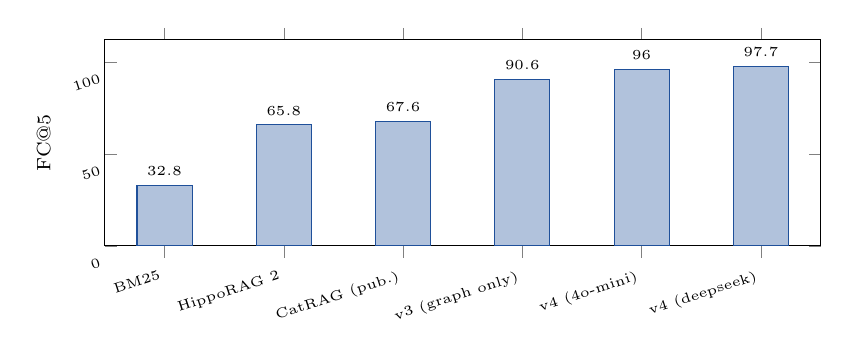
\begin{tikzpicture}
\begin{axis}[ybar, width=0.88\textwidth, height=42mm, bar width=7mm,
  symbolic x coords={BM25, HippoRAG 2, CatRAG (pub.), v3 (graph only), v4 (4o-mini), v4 (deepseek)},
  xtick=data, ymin=0, ymax=112, ylabel={\scriptsize FC@5}, nodes near coords,
  every node near coord/.append style={font=\tiny},
  tick label style={font=\tiny, rotate=18, anchor=north east}, label style={font=\tiny}]
\addplot[fill=azul!35, draw=azul] coordinates {(BM25,32.8) (HippoRAG 2,65.8) (CatRAG (pub.),67.6) (v3 (graph only),90.6) (v4 (4o-mini),96.0) (v4 (deepseek),97.7)};
\end{axis}
\end{tikzpicture}

\vspace{1mm}
\small
\begin{tabular}{lcccc}
\toprule
 & R@2 & R@5 & FC@5 & FC@10\\
\midrule
\hippo{} (its code) & $70.7$ & $85.9$ & $65.8$ & $71.7$\\
\sys{} v4 (\texttt{deepseek}) & $\mathbf{84.2}$ & $\mathbf{98.9}$ & $\mathbf{97.7}$ & $\mathbf{97.8}$\\
\bottomrule
\end{tabular}

\vspace{1mm}
\scriptsize Paired $\Delta\mathrm{FC@}5=+31.9$ $[+28.9,+34.9]$: wins $326$ /
loses $7$; all four types significant. \hippo{}'s own paper with a 7B GPU
encoder reports $\mathrm{R@}5=90.4$; here $98.9$ at a fraction of the cost.
\end{frame}

\begin{frame}{Case study: three mechanisms, stage by stage}
\centering\scriptsize
\emph{``Which film has the director who is older, God's Gift to Women or Aldri annet enn br\aa k?''}
--- gold: 2 films $+$ their directors (\textbf{M. Curtiz}, \textbf{E. Carlmar}).\quad
\colorbox{grisf!15}{\tiny inherited from \hippo{} unchanged}\ \
\colorbox{teja!15}{\tiny what each system changes}
\vspace{1mm}

\resizebox{0.99\textwidth}{!}{%
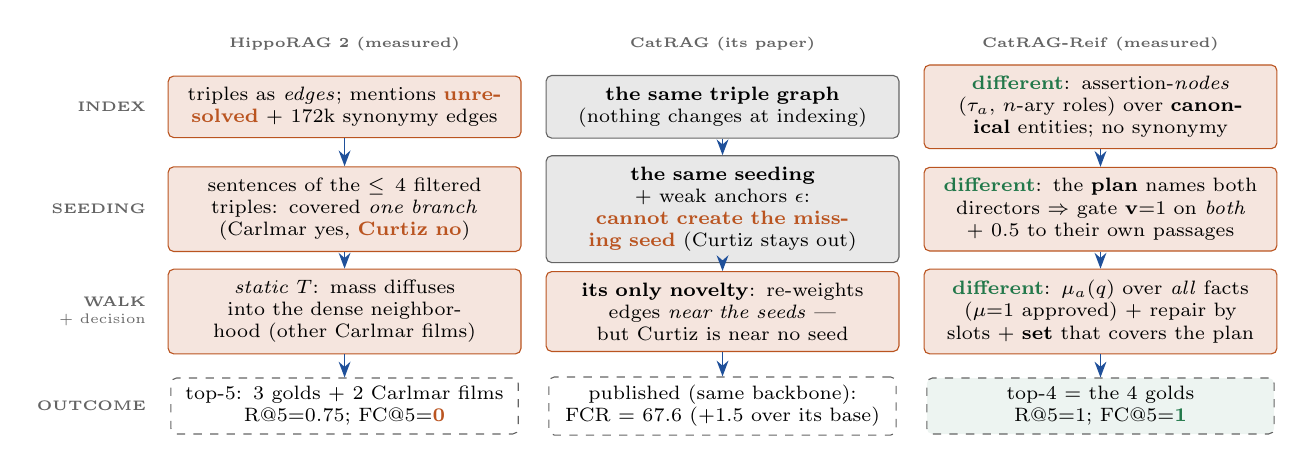
\begin{tikzpicture}[x=1mm, y=1mm, font=\tiny]
  \node[et, align=right, anchor=east] at (-2,42) {\textbf{INDEX}};
  \node[et, align=right, anchor=east] at (-2,29) {\textbf{SEEDING}};
  \node[et, align=right, anchor=east] at (-2,16) {\textbf{WALK}\\ $+$ decision};
  \node[et, align=right, anchor=east] at (-2,4)  {\textbf{OUTCOME}};
  \node[et] at (22,50)  {\textbf{\hippo{} (measured)}};
  \node[et] at (70,50)  {\textbf{CatRAG (its paper)}};
  \node[et] at (118,50) {\textbf{\sys{} (measured)}};
  \node[caja, fill=teja!15, draw=teja, text width=42mm] (i1) at (22,42)
    {triples as \emph{edges}; mentions \bad{unresolved} $+$ $172$k synonymy edges};
  \node[caja, fill=grisf!15, draw=grisf, text width=42mm] (i2) at (70,42)
    {\textbf{the same triple graph}\\ (nothing changes at indexing)};
  \node[caja, fill=teja!15, draw=teja, text width=42mm] (i3) at (118,42)
    {\good{different}: assertion-\emph{nodes} ($\tau_a$, $n$-ary roles) over \textbf{canonical} entities; no synonymy};
  \node[caja, fill=teja!15, draw=teja, text width=42mm] (s1) at (22,29)
    {sentences of the $\le4$ filtered triples: covered \emph{one branch}\\ (Carlmar yes, \bad{Curtiz no})};
  \node[caja, fill=grisf!15, draw=grisf, text width=42mm] (s2) at (70,29)
    {\textbf{the same seeding} $+$ weak anchors $\epsilon$:\\ \bad{cannot create the missing seed} (Curtiz stays out)};
  \node[caja, fill=teja!15, draw=teja, text width=42mm] (s3) at (118,29)
    {\good{different}: the \textbf{plan} names both directors $\Rightarrow$ gate $\mathbf v{=}1$ on \emph{both} $+$ $0.5$ to their own passages};
  \node[caja, fill=teja!15, draw=teja, text width=42mm] (p1) at (22,16)
    {\emph{static} $T$: mass diffuses into the dense neighborhood (other Carlmar films)};
  \node[caja, fill=teja!15, draw=teja, text width=42mm] (p2) at (70,16)
    {\textbf{its only novelty}: re-weights edges \emph{near the seeds} --- but Curtiz is near no seed};
  \node[caja, fill=teja!15, draw=teja, text width=42mm] (p3) at (118,16)
    {\good{different}: $\mu_a(q)$ over \emph{all} facts ($\mu{=}1$ approved) $+$ repair by slots $+$ \textbf{set} that covers the plan};
  \node[dato, text width=42mm] (r1) at (22,4)
    {top-5: 3 golds $+$ 2 Carlmar films\\ $\mathrm{R@}5{=}0.75$; $\mathrm{FC@}5{=}\bad{0}$};
  \node[dato, text width=42mm] (r2) at (70,4)
    {published (same backbone):\\ $\mathrm{FCR}=67.6$ ($+1.5$ over its base)};
  \node[dato, fill=verde!8, text width=42mm] (r3) at (118,4)
    {top-4 $=$ the 4 golds\\ $\mathrm{R@}5{=}1$; $\mathrm{FC@}5{=}\good{1}$};
  \draw[fl] (i1)--(s1); \draw[fl] (s1)--(p1); \draw[fl] (p1)--(r1);
  \draw[fl] (i2)--(s2); \draw[fl] (s2)--(p2); \draw[fl] (p2)--(r2);
  \draw[fl] (i3)--(s3); \draw[fl] (s3)--(p3); \draw[fl] (p3)--(r3);
\end{tikzpicture}}

\vspace{1mm}
\scriptsize Column reading: CatRAG changes \emph{one} stage and inherits
index and seeding ($+1.5$); \sys{} changes all four.
\end{frame}

\begin{frame}{The central finding: accumulation versus collapse with depth}
\begin{columns}[T]
\column{0.55\textwidth}
\centering
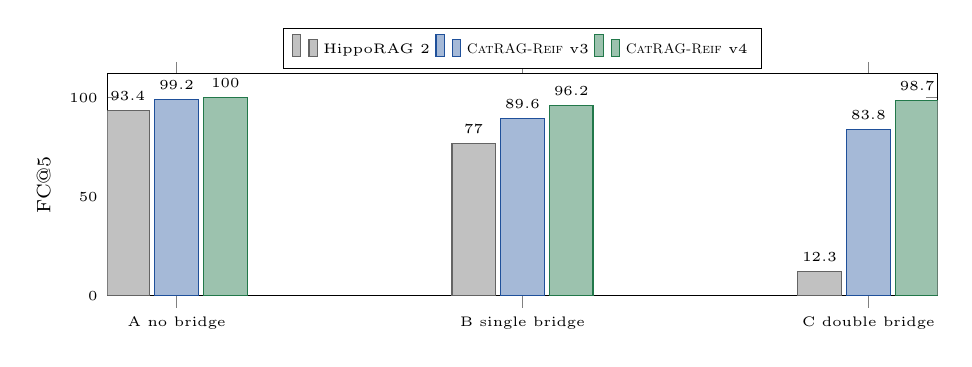
\begin{tikzpicture}
\begin{axis}[ybar, width=\textwidth, height=44mm, bar width=5.5mm,
  symbolic x coords={A no bridge, B single bridge, C double bridge},
  xtick=data, ymin=0, ymax=112, ylabel={\scriptsize FC@5},
  legend style={font=\tiny, at={(0.5,1.02)}, anchor=south, legend columns=3},
  nodes near coords, every node near coord/.append style={font=\tiny},
  tick label style={font=\tiny}, label style={font=\tiny}]
\addplot[fill=grisf!40, draw=grisf] coordinates {(A no bridge,93.4) (B single bridge,77.0) (C double bridge,12.3)};
\addplot[fill=azul!40, draw=azul] coordinates {(A no bridge,99.2) (B single bridge,89.6) (C double bridge,83.8)};
\addplot[fill=verde!45, draw=verde] coordinates {(A no bridge,100) (B single bridge,96.2) (C double bridge,98.7)};
\legend{\hippo{}, \sys{} v3, \sys{} v4}
\end{axis}
\end{tikzpicture}
\column{0.45\textwidth}
\textbf{Null model}: independent links
$\Rightarrow \mathrm{FC}\approx p^{\,|G_q|}$
\begin{center}\small
\begin{tabular}{lccc}
\toprule
 & C pred. & C obs. & ratio\\
\midrule
\hippo{} & $59.2$ & $12.3$ & \bad{$0.21$}\\
\sys{} v3 & $80.3$ & $83.8$ & \good{$1.04$}\\
\bottomrule
\end{tabular}
\end{center}
\footnotesize
v3 degrades by \emph{accumulation} ($\sim$5\% per link). \hippo{}
\emph{collapses}: fixed per-query resources shared across chains. The
planner \textbf{inverts the gradient}: with v4 the double chain becomes
the \emph{best} stratum ($98.7$).
\end{columns}
\end{frame}

\begin{frame}{The system's evolution: design by diagnosis}
\centering
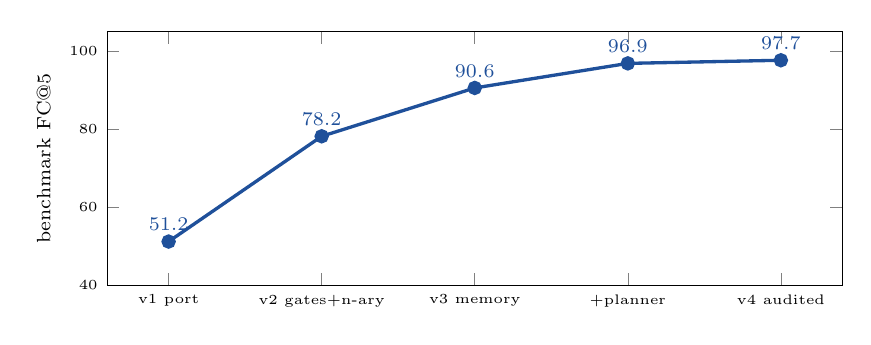
\begin{tikzpicture}
\begin{axis}[width=0.9\textwidth, height=48mm, ymin=40, ymax=105,
  symbolic x coords={v1 port, v2 gates+n-ary, v3 memory, +planner, v4 audited},
  xtick=data, ylabel={\scriptsize benchmark FC@5},
  nodes near coords, every node near coord/.append style={font=\scriptsize},
  tick label style={font=\tiny}, label style={font=\tiny}]
\addplot[mark=*, azul, very thick] coordinates {(v1 port,51.2) (v2 gates+n-ary,78.2) (v3 memory,90.6) (+planner,96.9) (v4 audited,97.7)};
\end{axis}
\end{tikzpicture}

\vspace{1mm}
\scriptsize
\begin{tabular}{lll}
\toprule
step & measured diagnosis of the predecessor & remedy\\
\midrule
$\to$v2 & filter used parametric knowledge; $n$-ary participants unreachable & few-shot filter, hard gate, $n$-ary roles\\
$\to$v3 & $57\%$ of failures were identity islands & canonical memory $+$ own-passage seeding\\
$\to$plan & filter \emph{saw} the bridge but did not select it ($12/15$) & analyst plan, repair hop, set packing\\
$\to$v4 & QID audit: $74$ over-merged entries; linker blind to variants & audited curation; name-to-name linker\\
\bottomrule
\end{tabular}

\vspace{1mm}
\scriptsize $+46$ FC@5 in four iterations --- every decision on held-out
probes, one benchmark measurement per configuration.
\end{frame}

\begin{frame}{Attribution I: component ablations (held-out probe)}
\begin{columns}[T]
\column{0.5\textwidth}
\centering
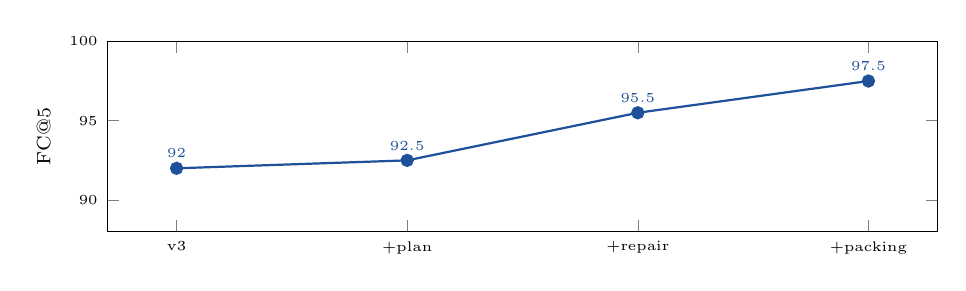
\begin{tikzpicture}
\begin{axis}[width=\textwidth, height=40mm, ymin=88, ymax=100,
  symbolic x coords={v3, +plan, +repair, +packing},
  xtick=data, ylabel={\scriptsize FC@5}, nodes near coords,
  every node near coord/.append style={font=\tiny},
  tick label style={font=\tiny}, label style={font=\tiny}]
\addplot[mark=*, azul, thick] coordinates {(v3,92.0) (+plan,92.5) (+repair,95.5) (+packing,97.5)};
\end{axis}
\end{tikzpicture}
\column{0.5\textwidth}
\footnotesize
The plan alone barely moves the aggregate ($+0.5$): its value is to
\emph{enable}
\begin{itemize}\footnotesize
\item the \textbf{repair hop} ($+3.0$; double chains $86\to96$) and
\item the \textbf{set packing} ($+1.5$; $+6$ FC@2 early ordering).
\end{itemize}
Transfers to HotpotQA's probe: repair $+2.0$ $[+0.5,+4.0]$, packing
$+4.0$ R@2 $[+1.5,+6.8]$.\\[1mm]
Planner-model sweep (probe FC@5): deepseek $97.5$ · gpt-oss-20B $97.0$ ·
gpt-4o $96.5$ · 4o-mini $96.0$ --- \good{the design, not the scale, carries
the gain}; a weak model (qwen-27B, $67.5$) marks the capability floor.
\end{columns}
\end{frame}

\begin{frame}{Attribution II: graph or planner? A no-graph control at identical budget}
\begin{columns}[T]
\column{0.55\textwidth}
\footnotesize
Same analyst, repair, packer, prompts, demos, budget --- over dense top-20
passages $+$ a title index; \textbf{no} assertions, memory, graph, walk.
\begin{center}\small
\begin{tabular}{lccc}
\toprule
benchmark & v4 & control & $\Delta$ [CI 95\%]\\
\midrule
2Wiki & $96.0$ & $83.3$ & \good{$+12.7$} $[+10.5,+14.9]$\\
HotpotQA & $90.2$ & $83.9$ & \good{$+6.3$} $[+4.1,+8.6]$\\
\bottomrule
\end{tabular}
\end{center}
\scriptsize Pre-registered criterion ($\ge5$, significant on both):
\good{met}. A post-hoc strengthened control still loses $9.6$/$5.1$.
\column{0.43\textwidth}
\footnotesize
\textbf{Where the control fails}: of the golds it misses (v4 finds),
$130/141$ are \bad{outside its top-20} --- failure of \emph{reach}, not
of ranking. The same planner reads ``\dots directed by Ben Holmes'' in
prose and writes $[X]$; as an atomic assertion it approves it and the
memory turns approval into retrieval.\\[1mm]
\textbf{Decomposition of the margin over CatRAG}: planner share /
representation share $= +15.7/+12.7$ (2Wiki), $+3.5/+6.3$ (HotpotQA).
The control alone already beats the published graph baselines on HotpotQA
($83.9$ vs $80.4$).
\end{columns}
\end{frame}

\begin{frame}{Generalization with a frozen configuration}
\begin{columns}[T]
\column{0.52\textwidth}
\textbf{HotpotQA} ($1{,}000\times9{,}811$), zero tuning:
\begin{center}\small
\begin{tabular}{lcc}
\toprule
 & R@5 & FC@5\\
\midrule
BM25 (ours) & $72.8$ & $49.5$\\
dense \texttt{te3-small} (pub.) & $81.3$ & $64.9$\\
\hippo{} (published) & $87.1$ & $75.5$\\
CatRAG (published) & $89.5$ & $80.4$\\
\sys{} v4 (\texttt{4o-mini}) & $94.7$ & $90.2$\\
\sys{} v4 (\texttt{deepseek}) & $\mathbf{96.0}$ & $\mathbf{93.0}$\\
\bottomrule
\end{tabular}
\end{center}
\column{0.46\textwidth}
\footnotesize
\begin{itemize}\footnotesize
\item $+6.5$ R@5 / $+12.6$ FC@5 over the best published graph system,
  with every dial, prompt and exemplar frozen from 2Wiki.
\item Same index recipe: $87{,}629$ assertions, $48{,}856$ entries,
  $146$k-node graph, ${\sim}\$4.7$ once.
\item Error profile unchanged in kind: $96/98$ residual failures are
  bridges; the missing gold sits at ranks 6--20 or beyond.
\end{itemize}
\end{columns}
\end{frame}

\begin{frame}{Why it works: each principle removes one dependency on depth}
\begin{enumerate}
\item \textbf{Identity in the index} (canonical memory): islands do not
  multiply with hops; thresholded synonymy does.
\item \textbf{Facts as first-class nodes}: mass travels \emph{through} the
  approved fact at full weight; qualifiers travel inside the unit.
\item \textbf{Resources that scale with the chain} (plan $\to$ repair $\to$
  packing): budget per slot, not per query --- hence the inverted gradient
  on double chains.
\end{enumerate}
\vspace{1mm}
\footnotesize The closed form makes the division of labor exact: the walk
diffuses; \emph{seeding} chains. The planner decides the seeds; the
representation makes every approved fact and discovered entity
\emph{reachable} (own passage) and \emph{preferable} ($\mu=1$).
\end{frame}

\begin{frame}{Limitations and ongoing work}
\begin{itemize}
\item \textbf{End-to-end answering} (EM/F1, Joint Success Rate) pending;
  published JSR references: $53.0$/$55.0$.
\item \textbf{MuSiQue} (labeled 2/3/4 hops): direct test of the
  multiplicative model and of multi-round repair; requires own-passage as a
  \emph{set} ($647$ repeated titles).
\item Inference stratum ($n{=}108$) not individually significant; single
  encoder untested for sensitivity.
\item Analyst prompt semantics (slots, $[X]$) defined partly by
  demonstration; a specification-first prompt is registered as an evolution
  for smaller models.
\item Clinical instantiation (the motivating deployment): unfilled slots
  $\to$ grounded abstention; packed sets $\to$ auditable evidence dossiers.
\end{itemize}
\end{frame}

\begin{frame}{Conclusions}
\begin{itemize}
\item Chain-level failure has \textbf{structural causes} --- unresolved
  identity and fixed per-query budgets --- and both are removable by design.
\item A retriever that resolves identity in the index, reifies facts into
  modulable nodes, and plans evidence with a bounded three-role LLM
  pipeline recovers complete chains: $\mathrm{FC@}5$
  \textbf{97.7} vs $65.8$/$67.6$ (2Wiki) and \textbf{93.0} vs $80.4$
  (HotpotQA, frozen).
\item The gains are \textbf{attributed} (ablations; no-graph control:
  representation $+12.7$/$+6.3$), \textbf{explained} (closed form:
  seeding chains, the walk diffuses) and \textbf{cheap}
  (${\sim}\$0.001$/query; open 20B planner nearly ties gpt-4o).
\item Everything is reproducible at zero cost: code, prompts, per-question
  outputs and caches at \texttt{github.com/bjur27r/hiv\_rag}
  (\texttt{eval-wiki2}).
\end{itemize}
\end{frame}

\end{document}
